\documentclass[aspectratio=169]{beamer}
\usepackage{amsmath}
\usepackage{amssymb}
\usepackage{tikz}
\usepackage{wasysym}
\usepackage{tikzsymbols}
\usepackage{xcolor}
\usepackage{animate}     % Option 1: play a PNG frame sequence
\usepackage{multimedia}  % Option 2: embed a video file (needs -shell-escape)
\usetikzlibrary{shapes,backgrounds,patterns}

% --- added for these slides -------------------------------------------------
\usepackage{pgfplots}
\pgfplotsset{compat=1.18, legend cell align=left}
\usetikzlibrary{arrows.meta,decorations.pathreplacing,calc,positioning}
\usepackage{listings}
\usepackage{booktabs}
% ----------------------------------------------------------------------------

% royalblue isn't a base xcolor name, so define it first (this is the default accent)
\definecolor{royalblue}{RGB}{65,105,225}

% ============================================================
%  ACCENT COLOR: change ONE line below to switch the theme
%  Choose one of: royalblue , red , black
% ============================================================
\colorlet{accent}{royalblue}
% \colorlet{accent}{red}
% \colorlet{accent}{black}
% ============================================================

% Use default theme with white background
\usetheme{default}

% Make everything white/black, with the chosen accent color for structure
\setbeamercolor{background canvas}{bg=white}
\setbeamercolor{normal text}{fg=black}
\setbeamercolor{structure}{fg=accent}
\setbeamercolor{frametitle}{fg=accent,bg=white}
\setbeamercolor{title}{fg=accent}
\setbeamercolor{section in toc}{fg=black}
\setbeamercolor{block title}{fg=black,bg=gray!10}
\setbeamercolor{block body}{fg=black,bg=gray!5}
\setbeamercolor{block title example}{fg=black,bg=green!10}
\setbeamercolor{block body example}{fg=black,bg=green!5}
\setbeamercolor{block title alerted}{fg=black,bg=red!10}
\setbeamercolor{block body alerted}{fg=black,bg=red!5}

\usepackage{scalerel}

\newcommand{\subsmall}[1]{_{\scaleto{#1}{4pt}}}
\newcommand{\supsmall}[1]{^{\scaleto{#1}{2pt}}}

% Remove navigation symbols
\setbeamertemplate{navigation symbols}{}

% Simple footline with page numbers (single definition)
\setbeamertemplate{footline}{
    \hfill\makebox[5pt]{%
        \scriptsize\insertframenumber}
    \hspace*{2em}
    \vspace{0.5cm}
}

% Custom command for colored boxes
\newcommand{\cbox}[2]{\colorbox{#1}{\ensuremath{\displaystyle #2}}}

% --- code listings (Python), coloured with the accent -----------------------
\lstdefinestyle{py}{
  language=Python,
  basicstyle=\ttfamily\footnotesize,
  keywordstyle=\color{accent}\bfseries,
  commentstyle=\color{gray}\itshape,
  stringstyle=\color{green!45!black},
  showstringspaces=false,
  columns=fullflexible,
  keepspaces=true,
  backgroundcolor=\color{gray!6},
  frame=single, rulecolor=\color{gray!30},
  xleftmargin=2pt, xrightmargin=2pt,
  escapeinside={(*}{*)}
}
\lstset{style=py}

% --- shared style for the small "what can go wrong" pictures -----------------
\pgfplotsset{
  miniplot/.style={
    width=4.0cm, height=3.0cm,
    axis lines=middle, xtick=\empty, ytick=\empty,
    samples=120, thick, clip=true
  }
}

\title{Root Finding I: Bracketing Methods}
\subtitle{Bisection and false position}
\author{Sharareh Sayyad}
\institute{Washington State University}
\date{\today}

\begin{document}

% Title Slide
\frame{\titlepage}

% Table of Contents
\begin{frame}{Outline}
\tableofcontents
\end{frame}

% ============================================================
\section{The root-finding problem}
% ============================================================

\begin{frame}{Root finding: solve $f(x) = 0$}
\begin{columns}[c]
\begin{column}{0.5\textwidth}
\small
A \textbf{root} (or zero) of $f$ is a number $r$ with $f(r) = 0$.

\vspace{0.2cm}
Almost any equation can be written this way:
\begin{itemize}
  \item $x^2 = 2 \quad\Longrightarrow\quad f(x) = x^2 - 2$
  \item $\cos x = x \quad\Longrightarrow\quad f(x) = \cos x - x$
\end{itemize}
\vspace{0.1cm}
\begin{block}{The problem}
Most equations have \textbf{no formula} for the root. We compute a sequence $x_1, x_2, \ldots \to r$ and stop when it is close enough.
\end{block}
\end{column}
\begin{column}{0.47\textwidth}
\centering
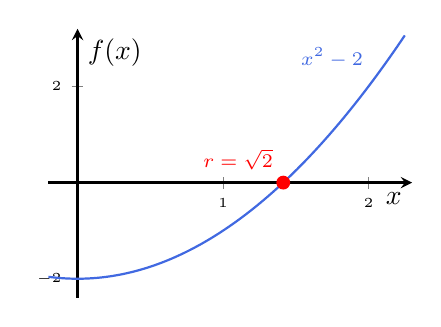
\begin{tikzpicture}
\begin{axis}[width=6.2cm, height=5cm, axis lines=middle, xmin=-0.2, xmax=2.3, ymin=-2.4, ymax=3.2,
  xtick={1,2}, ytick={-2,2}, samples=100, thick,
  tick label style={font=\tiny}, xlabel={$x$}, ylabel={$f(x)$},
  every axis x label/.style={at={(axis description cs:1,0.43)},anchor=north east},
  every axis y label/.style={at={(axis description cs:0.08,1)},anchor=north west}]
  \addplot[accent, domain=-0.2:2.25] {x^2-2};
  \fill[red] (axis cs:1.41421,0) circle (2.5pt);
  \node[red, font=\scriptsize, above left] at (axis cs:1.41421,0.05) {$r = \sqrt2$};
  \node[accent, font=\scriptsize] at (axis cs:1.75,2.6) {$x^2 - 2$};
\end{axis}
\end{tikzpicture}\\[2pt]
\scriptsize Today: methods that \textbf{never fail}\\ once we have a starting interval.
\end{column}
\end{columns}
\end{frame}

\begin{frame}{Bracketing: the Intermediate Value Theorem}
\begin{columns}[c]
\begin{column}{0.48\textwidth}
\small
\begin{block}{Intermediate Value Theorem}
If $f$ is \textbf{continuous} on $[a,b]$ and $f(a)$, $f(b)$ have \textbf{opposite signs}, then $f$ has at least one root in $(a,b)$.
\end{block}
\vspace{0.2cm}
Such an interval $[a,b]$ is called a \textbf{bracket}.

\vspace{0.2cm}
\begin{exampleblock}{Test for a bracket}
$f(a)$ and $f(b)$ have opposite signs, i.e.\ \texttt{np.sign(f(a)) != np.sign(f(b))}.
\end{exampleblock}
\vspace{0.1cm}
\scriptsize Intuition: a continuous curve cannot get from below the axis to above it without crossing it.
\end{column}
\begin{column}{0.5\textwidth}
\centering
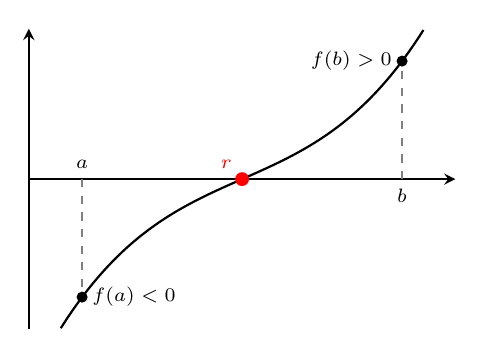
\begin{tikzpicture}
\begin{axis}[width=7cm, height=5.4cm, axis lines=middle, xmin=0, xmax=4, ymin=-1.6, ymax=1.6,
  xtick=\empty, ytick=\empty, samples=100, thick]
  \addplot[black, domain=0.3:3.7] {0.15*(x-2)^3+0.5*(x-2)};
  \draw[dashed, gray] (axis cs:0.5,0) -- (axis cs:0.5,-1.256);
  \draw[dashed, gray] (axis cs:3.5,0) -- (axis cs:3.5,1.256);
  \fill (axis cs:0.5,-1.256) circle (2pt) node[right, font=\scriptsize] {$f(a) < 0$};
  \fill (axis cs:3.5,1.256) circle (2pt) node[left, font=\scriptsize] {$f(b) > 0$};
  \node[above, font=\scriptsize] at (axis cs:0.5,0) {$a$};
  \node[below, font=\scriptsize] at (axis cs:3.5,0) {$b$};
  \fill[red] (axis cs:2,0) circle (2.5pt);
  \node[red, above left, font=\scriptsize] at (axis cs:2,0) {$r$};
\end{axis}
\end{tikzpicture}
\end{column}
\end{columns}
\end{frame}

\begin{frame}{Bracketing: what can go wrong}
\small Both conditions of the theorem matter. Always \textbf{plot $f$ first}.
\vspace{0.3cm}
\begin{columns}[T]
\begin{column}{0.32\textwidth}
\centering
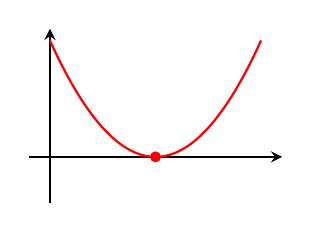
\begin{tikzpicture}
\begin{axis}[miniplot, width=4.8cm, height=3.8cm, xmin=-0.2, xmax=2.2, ymin=-0.4, ymax=1.1]
  \addplot[red, domain=0:2] {(x-1)^2};
  \fill[red] (axis cs:1,0) circle (2pt);
\end{axis}
\end{tikzpicture}\\[3pt]
\textbf{Root, no sign change}\\[2pt]
\scriptsize $f(x) = (x-1)^2$ touches the axis at $x = 1$ but never changes sign: there is no bracket, so bracketing methods cannot find this root.
\end{column}
\begin{column}{0.32\textwidth}
\centering
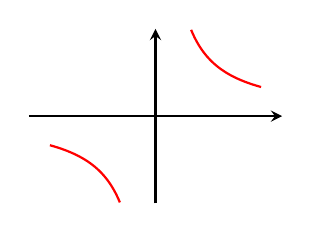
\begin{tikzpicture}
\begin{axis}[miniplot, width=4.8cm, height=3.8cm, xmin=-1.2, xmax=1.2, ymin=-3, ymax=3, restrict y to domain=-3:3]
  \addplot[red, domain=-1:-0.05] {1/x};
  \addplot[red, domain=0.05:1] {1/x};
\end{axis}
\end{tikzpicture}\\[3pt]
\textbf{Sign change, no root}\\[2pt]
\scriptsize $f(x) = 1/x$ on $[-1,1]$ changes sign, but $f$ is not continuous. Bisection happily ``converges'' to the jump at $x = 0$.
\end{column}
\begin{column}{0.32\textwidth}
\centering
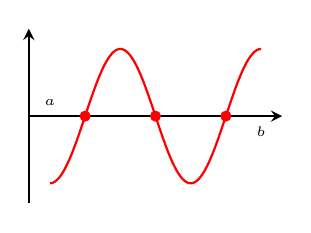
\begin{tikzpicture}
\begin{axis}[miniplot, width=4.8cm, height=3.8cm, xmin=0.2, xmax=3.8, ymin=-1.3, ymax=1.3]
  \addplot[red, domain=0.5:3.5] {-sin(deg(pi*x))};
  \node[font=\tiny, above] at (axis cs:0.5,0) {$a$};
  \node[font=\tiny, below] at (axis cs:3.5,0) {$b$};
  \fill[red] (axis cs:1,0) circle (2pt);
  \fill[red] (axis cs:2,0) circle (2pt);
  \fill[red] (axis cs:3,0) circle (2pt);
\end{axis}
\end{tikzpicture}\\[3pt]
\textbf{Several roots}\\[2pt]
\scriptsize With three roots in $[a,b]$ there is still a sign change, and the method finds \emph{one} of them. Which one depends on the bracket.
\end{column}
\end{columns}
\end{frame}

% ============================================================
\section{The bisection method}
% ============================================================

\begin{frame}{Bisection: halve the bracket}
\begin{columns}[c]
\begin{column}{0.44\textwidth}
\small
Start with a bracket $[a,b]$. Repeat:
\begin{enumerate}
  \item Take the midpoint $c = \dfrac{a+b}{2}$.
  \item If $f(a)$ and $f(c)$ have opposite signs, the root is in $[a,c]$: set $b \leftarrow c$.
  \item Otherwise it is in $[c,b]$: set $a \leftarrow c$.
\end{enumerate}
\vspace{0.1cm}
\begin{exampleblock}{Invariant}
After every step, $[a,b]$ is \textbf{still a bracket}, and it is \textbf{half as wide}.
\end{exampleblock}
\scriptsize Like guessing a number between 1 and 100 with ``higher / lower'' answers.
\end{column}
\begin{column}{0.54\textwidth}
\centering
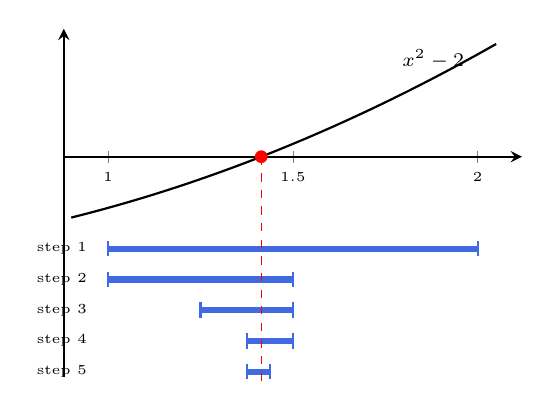
\begin{tikzpicture}
\begin{axis}[width=7.4cm, height=6cm, axis lines=middle, xmin=0.88, xmax=2.12, ymin=-4.3, ymax=2.5,
  xtick={1,1.5,2}, ytick=\empty, samples=80, thick, tick label style={font=\tiny},
  clip=false]
  \addplot[black, domain=0.9:2.05] {x^2-2};
  \node[font=\scriptsize] at (axis cs:1.88,1.9) {$x^2-2$};
  \fill[red] (axis cs:1.41421,0) circle (2.3pt);
  % nested brackets
  \draw[accent, line width=2.2pt] (axis cs:1,-1.8) -- (axis cs:2,-1.8);
  \draw[accent, thick] (axis cs:1,-1.65) -- (axis cs:1,-1.95);
  \draw[accent, thick] (axis cs:2,-1.65) -- (axis cs:2,-1.95);
  \node[font=\tiny, left] at (axis cs:0.97,-1.8) {step 1};
  \draw[accent, line width=2.2pt] (axis cs:1,-2.4) -- (axis cs:1.5,-2.4);
  \draw[accent, thick] (axis cs:1,-2.25) -- (axis cs:1,-2.55);
  \draw[accent, thick] (axis cs:1.5,-2.25) -- (axis cs:1.5,-2.55);
  \node[font=\tiny, left] at (axis cs:0.97,-2.4) {step 2};
  \draw[accent, line width=2.2pt] (axis cs:1.25,-3.0) -- (axis cs:1.5,-3.0);
  \draw[accent, thick] (axis cs:1.25,-2.85) -- (axis cs:1.25,-3.15);
  \draw[accent, thick] (axis cs:1.5,-2.85) -- (axis cs:1.5,-3.15);
  \node[font=\tiny, left] at (axis cs:0.97,-3.0) {step 3};
  \draw[accent, line width=2.2pt] (axis cs:1.375,-3.6) -- (axis cs:1.5,-3.6);
  \draw[accent, thick] (axis cs:1.375,-3.45) -- (axis cs:1.375,-3.75);
  \draw[accent, thick] (axis cs:1.5,-3.45) -- (axis cs:1.5,-3.75);
  \node[font=\tiny, left] at (axis cs:0.97,-3.6) {step 4};
  \draw[accent, line width=2.2pt] (axis cs:1.375,-4.2) -- (axis cs:1.4375,-4.2);
  \draw[accent, thick] (axis cs:1.375,-4.05) -- (axis cs:1.375,-4.35);
  \draw[accent, thick] (axis cs:1.4375,-4.05) -- (axis cs:1.4375,-4.35);
  \node[font=\tiny, left] at (axis cs:0.97,-4.2) {step 5};
  \draw[red, dashed, thin] (axis cs:1.41421,0) -- (axis cs:1.41421,-4.4);
\end{axis}
\end{tikzpicture}\\
\scriptsize Each bracket is half the previous one and always contains $\sqrt2$.
\end{column}
\end{columns}
\end{frame}

\begin{frame}[fragile]{Bisection in Python}
\begin{columns}[T]
\begin{column}{0.55\textwidth}
\begin{lstlisting}[basicstyle=\ttfamily\scriptsize]
def bisection(f, a, b, tol=1e-8, maxit=100):
    fa = f(a)
    if np.sign(fa) == np.sign(f(b)):
        raise ValueError("not a bracket")
    for n in range(maxit):
        c = a + (b - a)/2    # midpoint
        fc = f(c)            # the only new f-eval
        if (b - a)/2 < tol:  # error bound < tol
            return c
        if np.sign(fc) == np.sign(fa):
            a, fa = c, fc    # root in [c, b]
        else:
            b = c            # root in [a, c]
    return c
\end{lstlisting}
\vspace{-0.15cm}
\begin{block}{Floating point details}
\scriptsize
\texttt{a + (b-a)/2}: always lands inside $[a,b]$. \ \texttt{np.sign} instead of \texttt{fa*fc < 0}: the product can underflow to $0$.
\end{block}
\end{column}
\begin{column}{0.42\textwidth}
\begin{alertblock}{Why not stop when $f(c) = 0$?}
\footnotesize
\begin{itemize}
  \item $f(c)$ is itself rounded, so an \textbf{exact} $0$ almost never happens: the test is too strong.
  \item If it does happen, nothing breaks: $\mathrm{sign}(0) \ne \mathrm{sign}(f(a))$, so we keep $[a, c]$, which still contains the root $c$.
\end{itemize}
\end{alertblock}
\begin{block}{Why not $|f(c)| < \text{tol}$ either?}
\scriptsize
That measures the \textbf{residual}, not the \textbf{error}. For $f(x) = (x-1)^{10}$: \ $|f(1.1)| = 10^{-10}$, yet $1.1$ is $0.1$ away from the root.\\[3pt]
Bisection gives a true error bound for free: stop when $(b-a)/2 < \text{tol}$.
\end{block}
\end{column}
\end{columns}
\end{frame}

\begin{frame}{Example: $\sqrt2$ by bisection, $f(x) = x^2 - 2$ on $[1,2]$}
\begin{columns}[c]
\begin{column}{0.64\textwidth}
\centering
\footnotesize
\setlength{\tabcolsep}{3.5pt}
\begin{tabular}{rcccrc}
\toprule
$n$ & $a$ & $b$ & $c$ & $f(c)$ & $|c - \sqrt2|$ \\
\midrule
1 & 1.000000 & 2.000000 & 1.500000 & $+0.2500$ & $8.6\times10^{-2}$ \\
2 & 1.000000 & 1.500000 & 1.250000 & $-0.4375$ & $1.6\times10^{-1}$ \\
3 & 1.250000 & 1.500000 & 1.375000 & $-0.1094$ & $3.9\times10^{-2}$ \\
4 & 1.375000 & 1.500000 & 1.437500 & $+0.0664$ & $2.3\times10^{-2}$ \\
5 & 1.375000 & 1.437500 & 1.406250 & $-0.0225$ & $8.0\times10^{-3}$ \\
6 & 1.406250 & 1.437500 & 1.421875 & $+0.0217$ & $7.7\times10^{-3}$ \\
7 & 1.406250 & 1.421875 & 1.414062 & $-0.0004$ & \cbox{green!15}{1.5\times10^{-4}} \\
8 & 1.414062 & 1.421875 & 1.417969 & $+0.0106$ & \cbox{red!15}{3.8\times10^{-3}} \\
\bottomrule
\end{tabular}
\end{column}
\begin{column}{0.33\textwidth}
\small
\begin{itemize}
  \item The \textbf{sign} of $f(c)$ decides which half to keep; its size is ignored.
  \item The error does \textbf{not} decrease every step: step 7 is lucky, step 8 is worse.
  \item What \emph{does} shrink every step is the \textbf{bracket width}: $1, \tfrac12, \tfrac14, \ldots$
\end{itemize}
\end{column}
\end{columns}
\end{frame}

\begin{frame}{How fast? A guaranteed error bound}
\begin{columns}[T]
\begin{column}{0.52\textwidth}
\small
After $n$ steps the midpoint $c_n$ satisfies
\[
|c_n - r| \;\le\; \frac{b-a}{2^{\,n}} .
\]
\begin{itemize}
  \item Linear convergence with $\rho = \tfrac12$: one \textbf{bit} per step, one decimal digit every $\log_2 10 \approx 3.3$ steps.
  \item Known \textbf{before} we start, whatever $f$ is.
\end{itemize}
\begin{block}{Number of steps for tolerance tol}
\[
\frac{b-a}{2^{\,n}} \le \text{tol}
\quad\Longleftrightarrow\quad
n \ge \log_2\!\frac{b-a}{\text{tol}}
\]
\end{block}
\end{column}
\begin{column}{0.45\textwidth}
\begin{exampleblock}{Example}
\footnotesize $[1,2]$, tol $= 10^{-6}$: \ $n \ge \log_2 10^6 \approx 19.9$, so \textbf{20 steps}.
\end{exampleblock}
\vspace{0.1cm}
\begin{block}{Cost in Big-$O$ terms}
\footnotesize One $f$-evaluation per step, so cost $=$ number of steps:
\[
n = \underbrace{\log_2(b-a)}_{\text{constant}} + \log_2\frac{1}{\text{tol}}
\]
\[
\Longrightarrow\quad \text{cost} = O\big(\log(1/\text{tol})\big).
\]
10 times more accuracy costs only $\log_2 10 \approx 3.3$ more steps.
\end{block}
\end{column}
\end{columns}
\end{frame}

% ============================================================
\section{The false position method}
% ============================================================

\begin{frame}{False position: use the secant line}
\begin{columns}[c]
\begin{column}{0.5\textwidth}
\small
Bisection ignores the \emph{values} of $f$. If $|f(a)|$ is small, the root is probably close to $a$.

\vspace{0.2cm}
\textbf{Idea:} replace $f$ by the straight line through $(a, f(a))$ and $(b, f(b))$, and take its zero:
\[
c = b - f(b)\,\frac{b - a}{f(b) - f(a)} = \frac{a\,f(b) - b\,f(a)}{f(b) - f(a)}
\]
Then keep the half with the sign change, exactly as in bisection.

\vspace{0.15cm}
\begin{exampleblock}{In code}
Only the line for \texttt{c} changes (and we keep \texttt{fb} too). The bracket is still guaranteed.
\end{exampleblock}
\end{column}
\begin{column}{0.47\textwidth}
\centering
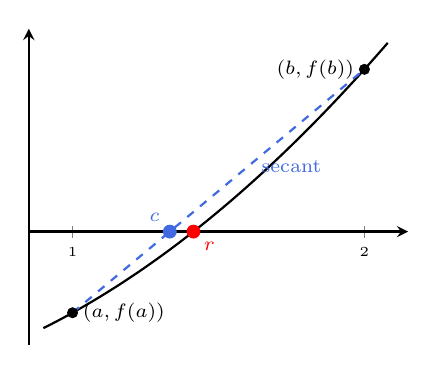
\begin{tikzpicture}
\begin{axis}[width=6.4cm, height=5.6cm, axis lines=middle, xmin=0.85, xmax=2.15, ymin=-1.4, ymax=2.5,
  xtick={1,2}, ytick=\empty, samples=80, thick, tick label style={font=\tiny}, clip=false]
  \addplot[black, domain=0.9:2.08] {x^2-2};
  \addplot[accent, dashed, domain=1:2] {3*x-4};
  \fill (axis cs:1,-1) circle (2pt) node[right, font=\scriptsize] {$(a, f(a))$};
  \fill (axis cs:2,2) circle (2pt) node[left, font=\scriptsize] {$(b, f(b))$};
  \fill[accent] (axis cs:1.3333,0) circle (2.5pt);
  \node[accent, font=\scriptsize, above left] at (axis cs:1.3333,0) {$c$};
  \fill[red] (axis cs:1.41421,0) circle (2.5pt);
  \node[red, font=\scriptsize, below right] at (axis cs:1.41421,0) {$r$};
  \node[accent, font=\scriptsize] at (axis cs:1.75,0.8) {secant};
\end{axis}
\end{tikzpicture}\\[2pt]
\scriptsize For $x^2-2$ on $[1,2]$: \ $c = \dfrac{1\cdot 2 - 2\cdot(-1)}{2-(-1)} = \tfrac43 \approx 1.333$.
\end{column}
\end{columns}
\end{frame}

\begin{frame}{Example: $\sqrt2$ by false position, same $f$ and bracket}
\begin{columns}[c]
\begin{column}{0.58\textwidth}
\centering
\small
\begin{tabular}{rcccc}
\toprule
$n$ & $a$ & $b$ & $c$ & $|c - \sqrt2|$ \\
\midrule
1 & 1.000000 & \cbox{accent!15}{2} & 1.333333 & $8.1\times10^{-2}$ \\
2 & 1.333333 & \cbox{accent!15}{2} & 1.400000 & $1.4\times10^{-2}$ \\
3 & 1.400000 & \cbox{accent!15}{2} & 1.411765 & $2.4\times10^{-3}$ \\
4 & 1.411765 & \cbox{accent!15}{2} & 1.413793 & $4.2\times10^{-4}$ \\
5 & 1.413793 & \cbox{accent!15}{2} & 1.414141 & $7.2\times10^{-5}$ \\
6 & 1.414141 & \cbox{accent!15}{2} & 1.414201 & $1.2\times10^{-5}$ \\
\bottomrule
\end{tabular}
\end{column}
\begin{column}{0.39\textwidth}
\small
\begin{itemize}
  \item Error shrinks by $\rho \approx 0.17$ each step: \textbf{linear}, but faster than bisection here.
  \item The endpoint $b = 2$ \textbf{never moves}: the bracket width tends to $2 - \sqrt2 \approx 0.59$, not to $0$.
  \item Error is below $10^{-6}$ after 8 steps (bisection: 19).
\end{itemize}
\end{column}
\end{columns}
\end{frame}

\begin{frame}{When false position is slow: the stuck endpoint}
\begin{columns}[c]
\begin{column}{0.42\textwidth}
\small
$f(x) = x^{10} - 1$ on $[0, 1.3]$, root $r = 1$.
\begin{itemize}\footnotesize
  \item $f$ is very flat on the left and steep on the right, so every secant line crosses the axis far to the left of $r$.
  \item $f(c_k) < 0$ every time, so $a$ moves and $b = 1.3$ is never replaced: steps of only $\approx 0.08$.
\end{itemize}
\centering
\begin{tabular}{lr}
\toprule
method & steps to $10^{-6}$ \\
\midrule
bisection & 20 \\
false position & 61 \\
\bottomrule
\end{tabular}

\vspace{0.05cm}
\begin{alertblock}{Lesson}
\scriptsize ``Smarter'' is not always faster: one stuck endpoint can make false position much slower than bisection.
\end{alertblock}
\end{column}
\begin{column}{0.56\textwidth}
\centering
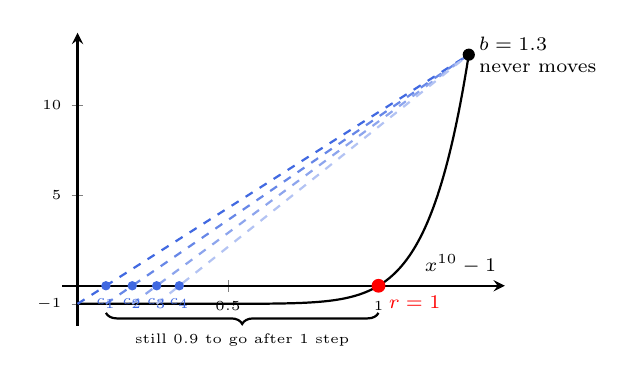
\begin{tikzpicture}
\begin{axis}[width=7.2cm, height=5.3cm, axis lines=middle, xmin=-0.05, xmax=1.42, ymin=-2.2, ymax=14,
  xtick={0.5,1}, ytick={-1,5,10}, samples=200, thick, tick label style={font=\tiny}, clip=false]
  \addplot[black, domain=0:1.3] {x^10-1};
  \node[font=\scriptsize, right] at (axis cs:1.12,1.2) {$x^{10}-1$};
  % secant lines from the stuck endpoint b = 1.3
  \addplot[accent, dashed, domain=0:1.3] {-1 + (12.7858+1)*(x-0)/1.3};
  \addplot[accent!80, dashed, domain=0.0943:1.3] {-1 + (12.7858+1)*(x-0.0943)/(1.3-0.0943)};
  \addplot[accent!60, dashed, domain=0.1818:1.3] {-1 + (12.7858+1)*(x-0.1818)/(1.3-0.1818)};
  \addplot[accent!40, dashed, domain=0.2629:1.3] {-1 + (12.7858+1)*(x-0.2629)/(1.3-0.2629)};
  \fill (axis cs:1.3,12.7858) circle (2.2pt) node[right, font=\scriptsize, align=left] {$b = 1.3$\\never moves};
  \foreach \c/\k in {0.0943/1, 0.1818/2, 0.2629/3, 0.3381/4} {
    \edef\tmp{\noexpand\fill[accent] (axis cs:\c,0) circle (1.7pt);}\tmp
  }
  \node[accent, font=\tiny, below] at (axis cs:0.0943,-0.15) {$c_1$};
  \node[accent, font=\tiny, below] at (axis cs:0.1818,-0.15) {$c_2$};
  \node[accent, font=\tiny, below] at (axis cs:0.2629,-0.15) {$c_3$};
  \node[accent, font=\tiny, below] at (axis cs:0.3381,-0.15) {$c_4$};
  \fill[red] (axis cs:1,0) circle (2.5pt);
  \node[red, font=\scriptsize, below right] at (axis cs:1,0) {$r = 1$};
  \draw[decorate, decoration={brace, amplitude=4pt, mirror}] (axis cs:0.0943,-1.5) -- (axis cs:1,-1.5)
     node[midway, below=4pt, font=\tiny] {still $0.9$ to go after 1 step};
\end{axis}
\end{tikzpicture}
\end{column}
\end{columns}
\end{frame}

% ============================================================
\section{Comparing and stopping}
% ============================================================

\begin{frame}{Bisection vs.\ false position}
\begin{columns}[c]
\begin{column}{0.5\textwidth}
\centering
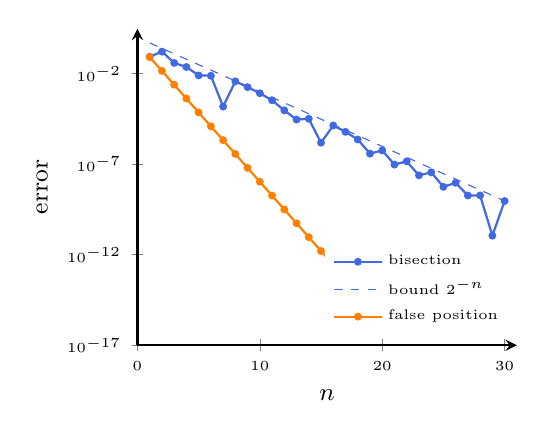
\begin{tikzpicture}
\begin{axis}[width=6.4cm, height=5.6cm, ymode=log, axis lines=left,
  xmin=0, xmax=31, ymin=1e-17, ymax=3, xlabel={$n$}, ylabel={error},
  thick, tick label style={font=\tiny}, label style={font=\small},
  legend style={font=\tiny, draw=none, at={(0.99,0.03)}, anchor=south east}]
  \addplot[accent, mark=*, mark size=1pt] coordinates {(1,0.0858) (2,0.164) (3,0.0392) (4,0.0233) (5,0.00796) (6,0.00766) (7,0.000151) (8,0.00376) (9,0.0018) (10,0.000826) (11,0.000337) (12,9.31e-05) (13,2.9e-05) (14,3.2e-05) (15,1.53e-06) (16,1.37e-05) (17,6.1e-06) (18,2.29e-06) (19,3.82e-07) (20,5.72e-07) (21,9.5e-08) (22,1.43e-07) (23,2.42e-08) (24,3.54e-08) (25,5.6e-09) (26,9.3e-09) (27,1.85e-09) (28,1.87e-09) (29,1.12e-11) (30,9.2e-10)};
  \addlegendentry{bisection}
  \addplot[accent, dashed, thin, domain=1:30, samples=30] {2^(-x)};
  \addlegendentry{bound $2^{-n}$}
  \addplot[orange, mark=*, mark size=1pt] coordinates {(1,0.0809) (2,0.0142) (3,0.00245) (4,0.00042) (5,7.21e-05) (6,1.24e-05) (7,2.12e-06) (8,3.64e-07) (9,6.25e-08) (10,1.07e-08) (11,1.84e-09) (12,3.16e-10) (13,5.42e-11) (14,9.3e-12) (15,1.59e-12) (16,2.74e-13) (17,4.71e-14) (18,8.22e-15) (19,1.55e-15) (20,2.22e-16)};
  \addlegendentry{false position}
\end{axis}
\end{tikzpicture}\\[2pt]
\scriptsize $x^2-2$ on $[1,2]$. Both are straight lines on \texttt{semilogy}: linear convergence.
\end{column}
\begin{column}{0.48\textwidth}
\centering
\scriptsize
\setlength{\tabcolsep}{3pt}
\begin{tabular}{lcc}
\toprule
 & bisection & false position \\
\midrule
needs a bracket & yes & yes \\
always converges & yes & yes \\
rate (linear) & $\rho = \tfrac12$ & $\rho$ depends on $f$ \\
error bound in advance & yes & no \\
bracket width $\to 0$ & yes & not always \\
$f$-evaluations per step & 1 & 1 \\
\bottomrule
\end{tabular}

\vspace{0.3cm}
\begin{block}{Bracketing = reliable, not fast}
\small Neither method can fail once you have a bracket. The price is speed: both converge only linearly.
\end{block}
\end{column}
\end{columns}
\end{frame}

\begin{frame}{When do we stop?}
\begin{columns}[T]
\begin{column}{0.5\textwidth}
\small
Three common tests (use more than one):
\begin{enumerate}
  \item \textbf{Bracket width:} $(b - a)/2 < \text{tol}$.\\
        \scriptsize Gives a true error bound for bisection, but may \textbf{never} trigger for false position.\small
  \item \textbf{Step size:} $|c_n - c_{n-1}| < \text{tol}$.\\
        \scriptsize Works for both; not a guarantee.\small
  \item \textbf{Residual:} $|f(c)| < \text{tol}_f$.\\
        \scriptsize Depends on the scale of $f$: compare $f$ and $10^6 f$.\small
\end{enumerate}
\vspace{0.1cm}
Always add a \textbf{maximum number of iterations}.
\end{column}
\begin{column}{0.47\textwidth}
\begin{alertblock}{Floating point floor}
\small Below $\text{tol} \approx 10^{-16}\,|r|$ there are no more floats between $a$ and $b$: the midpoint equals $a$ or $b$, and the loop runs forever without \texttt{maxit}.
\end{alertblock}
\vspace{0.1cm}
\begin{exampleblock}{Practical recipe}
\small
\begin{itemize}
  \item Plot $f$; choose a bracket with a sign change.
  \item Pick a \textbf{relative} tolerance, e.g.\ $10^{-10}|c|$.
  \item Stop on width or step size, cap with \texttt{maxit}.
\end{itemize}
\end{exampleblock}
\end{column}
\end{columns}
\end{frame}

% ============================================================
\section{Summary}
% ============================================================

\begin{frame}{Summary}
\begin{columns}[T]
\begin{column}{0.33\textwidth}
\begin{block}{Bracketing}
\scriptsize
\begin{itemize}
  \item root: $f(r) = 0$
  \item bracket: $f(a)$, $f(b)$ of opposite sign, $f$ continuous
  \item the bracket always holds a root
\end{itemize}
\end{block}
\end{column}
\begin{column}{0.33\textwidth}
\begin{block}{Bisection}
\scriptsize
\begin{itemize}
  \item $c = a + (b-a)/2$
  \item error $\le (b-a)/2^n$
  \item linear, $\rho = \tfrac12$
  \item steps $= \lceil \log_2((b-a)/\text{tol}) \rceil$
\end{itemize}
\end{block}
\end{column}
\begin{column}{0.33\textwidth}
\begin{block}{False position}
\scriptsize
\begin{itemize}
  \item $c$ = zero of the secant line
  \item linear, $\rho$ depends on $f$
  \item often faster, can be much slower
  \item one endpoint may get stuck
\end{itemize}
\end{block}
\end{column}
\end{columns}
\vspace{0.4cm}
\centering
\small Both: guaranteed to converge, one $f$-evaluation per step, limited by machine epsilon.\\[3pt]
\scriptsize Next lecture: methods that do not need a bracket.
\end{frame}

% ============================================================
\section{The Illinois method}
% ============================================================

\begin{frame}{Fixing the stuck endpoint: the Illinois method}
\begin{columns}[T]
\begin{column}{0.52\textwidth}
\begin{block}{Illinois = false position + one rule}
\footnotesize If the same endpoint is kept in \textbf{two steps in a row}, halve its stored function value (e.g.\ $f(b) \leftarrow f(b)/2$) before the next secant step.
\end{block}
\scriptsize
\textbf{One step:}
\begin{enumerate}
  \item $c = \frac{a f(b) - b f(a)}{f(b) - f(a)}$ as in false position; compute $f(c)$.
  \item Replace the endpoint whose $f$ has the sign of $f(c)$.
  \item Same side replaced as in the last step (track \texttt{side} $=\pm1$)? Halve the stored $f$ of the \emph{other} endpoint.
\end{enumerate}
\textbf{Why it is safe:} halving changes the \emph{size} of $f(b)$, not its \emph{sign}: $[a,b]$ stays a bracket. Still one $f$-evaluation per step; the convergence becomes \textbf{superlinear} (order $\approx 1.44$).
\end{column}
\begin{column}{0.45\textwidth}
\centering
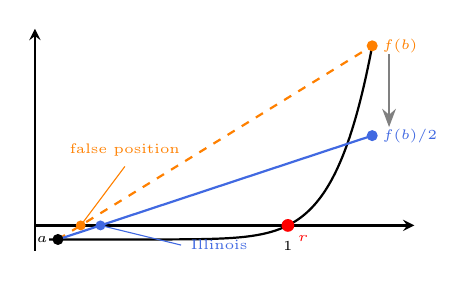
\begin{tikzpicture}
\begin{axis}[width=6.4cm, height=4.4cm, axis lines=middle, xmin=0.1, xmax=1.45, ymin=-1.8, ymax=14,
  xtick={1}, ytick=\empty, samples=200, thick, tick label style={font=\tiny}, clip=false]
  \addplot[black, domain=0.15:1.3] {x^10-1};
  \addplot[orange, dashed, domain=0.1818:1.3] {-1 + (12.7858+1)*(x-0.1818)/(1.3-0.1818)};
  \addplot[accent, domain=0.1818:1.3] {-1 + (6.3929+1)*(x-0.1818)/(1.3-0.1818)};
  \fill (axis cs:0.1818,-1) circle (2pt) node[left, font=\tiny] {$a$};
  \fill[orange] (axis cs:1.3,12.7858) circle (2pt) node[right, font=\tiny] {$f(b)$};
  \fill[accent] (axis cs:1.3,6.3929) circle (2pt) node[right, font=\tiny] {$f(b)/2$};
  \draw[-{Stealth}, gray] (axis cs:1.36,12.2) -- (axis cs:1.36,7.0);
  \fill[orange] (axis cs:0.2629,0) circle (1.8pt);
  \fill[accent] (axis cs:0.3331,0) circle (1.8pt);
  \draw[orange, thin] (axis cs:0.2629,0) -- (axis cs:0.42,4.2) node[above, font=\tiny] {false position};
  \draw[accent, thin] (axis cs:0.3331,0) -- (axis cs:0.62,-1.4) node[right, font=\tiny] {Illinois};
  \fill[red] (axis cs:1,0) circle (2.3pt);
  \node[red, font=\tiny, below right] at (axis cs:1,0) {$r$};
\end{axis}
\end{tikzpicture}\\[1pt]
\scriptsize $x^{10}-1$, step 3: the halved $f(b)$ tilts the line and pushes $c$ towards $r$.\\[5pt]
\footnotesize
\begin{tabular}{lr}
\toprule
$x^{10} - 1$ on $[0, 1.3]$ & steps to $10^{-6}$ \\
\midrule
bisection & 20 \\
false position & 61 \\
Illinois & \cbox{green!15}{13} \\
\bottomrule
\end{tabular}\\[4pt]
\scriptsize You will implement it in the notebook.
\end{column}
\end{columns}
\end{frame}

\end{document}
